%!TEX TS-program = xelatex
\documentclass[]{friggeri-cv}
\usepackage{afterpage}
\usepackage{hyperref}
\usepackage{color}
\usepackage{xcolor}
\usepackage{smartdiagram}
\usepackage{fontspec}
% if you want to add fontawesome package
% you need to compile the tex file with LuaLaTeX
% References:
%   http://texdoc.net/texmf-dist/doc/latex/fontawesome/fontawesome.pdf
%   https://www.ctan.org/tex-archive/fonts/fontawesome?lang=en
%\usepackage{fontawesome}
\usepackage{metalogo}
\usepackage{dtklogos}
\usepackage[utf8]{inputenc}
\usepackage{tikz}
\usetikzlibrary{mindmap,shadows}
\hypersetup{
    pdftitle={},
    pdfauthor={},
    pdfsubject={},
    pdfkeywords={},
    colorlinks=false,           % no lik border color
    allbordercolors=white       % white border color for all
}
\smartdiagramset{
    bubble center node font = \footnotesize,
    bubble node font = \footnotesize,
    % specifies the minimum size of the bubble center node
    bubble center node size = 0.5cm,
    %  specifies the minimum size of the bubbles
    bubble node size = 0.5cm,
    % specifies which is the distance among the bubble center node and the other bubbles
    distance center/other bubbles = 0.3cm,
    % sets the distance from the text to the border of the bubble center node
    distance text center bubble = 0.5cm,
    % set center bubble color
    bubble center node color = pblue,
    % define the list of colors usable in the diagram
    set color list = {lightgray, materialcyan, orange, green, materialorange, materialteal, materialamber, materialindigo, materialgreen, materiallime},
    % sets the opacity at which the bubbles are shown
    bubble fill opacity = 0.4,
    % sets the opacity at which the bubble text is shown
    bubble text opacity = 0.8,
}

\addbibresource{bibliography.bib}
\RequirePackage{xcolor}
\definecolor{pblue}{HTML}{0395DE}

\begin{document}
\header{Rahul}{ Patel}
      {Electronics circuit engineer \& Mathematician}
      
% Fake text to add separator      
\fcolorbox{white}{gray}{\parbox{\dimexpr\textwidth-2\fboxsep-2\fboxrule}{%
.....
}}

% In the aside, each new line forces a line break
\begin{aside}
  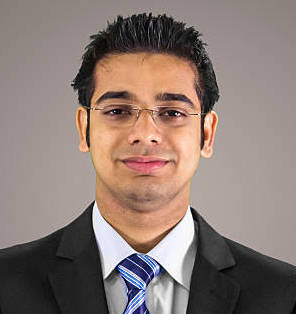
\includegraphics[scale=0.25]{img/image2.jpg}
  \section{\large Gender : Male}
  \section{\large Age : 40-45 years}
  \section{\large Email: samir.al@gmail.com}
  \section{\large Country: India}
   ~ 
  % use  \hspace{} or \vspace{} to change bubble size, if needed
%   \section{Interests}
%     \smartdiagram[bubble diagram]{
%         \textbf{Quantum}\\\textbf{Mechanics},
%         \textbf{Data}\\\textbf{Science},
%         \textbf{Electro-}\\\textbf{Magnetics},
%         \textbf{Cosmology},
%         \textbf{Quantum}\\\textbf{Computing},
%         \textbf{Research} 
%     }
    % ~
  \section{Skills}
    \smartdiagram[bubble diagram]{
        \textbf{Team}\\\textbf{Player},
        \textbf{Initiative},
        \textbf{Curiosity},
        \textbf{Problem}\\\textbf{Solving},
        \textbf{\vspace{2mm}Manage\vspace{2mm}},
        \textbf{Organize}
    }
    ~
\end{aside}
~
\section{Experience}
Rahul Patel is an Electronics circuit design engineer at Rambus Chip Technologies (India) Private Limited. He is graduated in Electrical Engineering with specialization Electronic Systems from 'Indian Institute of Technology Bombay - India. He has been remain close to Mathematics for more than 5 years. As an electronics circuit design engineers, he uses mathematics in electric circuit simulation using MATHEMATICA Software. 

\section{Interest}
His interests are in solving mathematical equations. He is already doing that using using MATHEMATICA Software.  He has used or studied many irrational numbers but mostly during his education period. He is familiar with Siver Ratio Number but never used practically. He knows real-life application that uses irrational numbers. He is open to work with Silver Ratio Number in future if required.

\section{Likes|Dislikes}
He like to push the boundaries of what is possible. He is likes to learn new things, in-fact he always keep his self busy learning new things. He likes to give suggestions on any mathematical calculations. He do not like to work with a person who is not self motivated.

\section{Business Values}
He believe that some day he will become an expert in solving mathematical problems. He thinks that his such expertises can help his company in research and development work.

\end{document}
